\documentclass[10pt]{beamer}

\usepackage{fontspec}
\usepackage{xunicode}
\usepackage{xltxtra}
\setsansfont{FreeSans}
\setmonofont{DejaVuSansMono}

\usepackage{listings}
\usepackage{textpos}
\usepackage{tikz}
\usepackage{minted}

\setbeamertemplate{footline}[frame]
\setbeamertemplate{items}[default]
\usetheme{Warsaw}
\usecolortheme{beaver}
\setbeamertemplate{itemize items}[default]
\setbeamertemplate{navigation symbols}{}
\setbeamertemplate{footline}[frame number]
\lstset{columns=fixed}
\setbeamerfont*{block body}{series=\tt}
\definecolor{lightgray}{rgb}{0.9,0.9,0.9}
\definecolor{midgray}{rgb}{0.5,0.5,0.5}

\newcommand{\light}[1]{\textcolor{gray}{\footnotesize{#1}}}
\newcommand{\code}[4]{\inputminted[linenos, frame=none, firstline=#2, lastline=#3,
  framesep=10pt, bgcolor=lightgray]{#4}{#1}}

\title[Об ошибках]{Alternatives in Error Handling}
\author{Dmitry Groshev}
\date{
\includegraphics[height=3cm]{stadshuset-townhall2}\\28.05.2012}
\institute{Erlang User Conference 2012}

% \addtobeamertemplate{frametitle}{}{%
% \begin{textblock*}{100mm}(1\textwidth,-0.7cm)
% 
\includegraphics[height=0.6cm]{stadshuset-townhall2}
% \end{textblock*}}

\begin{document}
\renewcommand*{\inserttotalframenumber}{\pageref{lastframe}}
\begin{frame}
\titlepage
\end{frame}

\begin{frame}{What's it all about}
  \begin{itemize}
  \item error handling is easy in Erlang
  \item case/try/catch/happy path coding/let it crash
  \item error handling is hard in Erlang
  \item dark side of Erlang
  \end{itemize}
\end{frame}

\begin{frame}{What's it all about}
  \begin{center}
    \code{code.erl}{1}{17}{erlang}
  \end{center}
\end{frame}

\begin{frame}{Not a real solution}
  \code{code.erl}{19}{29}{erlang}
  \begin{itemize}
  \item Still messy
  \item Nonsensical function names
  \item Lot of noise
  \end{itemize}
\end{frame}

\begin{frame}{Validators}
  \begin{itemize}
  \item XML Schema
  \item JSON Schema
  \item Sheriff
  \end{itemize}
\end{frame}

\begin{frame}{Meet Sheriff!}
  \begin{center}
    \Large
    Sheriff: https://github.com/extend/sheriff
  \end{center}
\end{frame}

\begin{frame}{Sheriff}
  \code{code.erl}{31}{37}{erlang}
\end{frame}

\begin{frame}{Still not good enough}
  \code{code.erl}{39}{46}{erlang}
\end{frame}

\begin{frame}{Expressiveness problem}
  \begin{itemize}
  \item<1-> IP: 183.234.123.93
  \item<1-> 4 numbers and dots?
  \item<2-> IPv6: E3D7:0000:0000:0000:51F4:9BC8:C0A8:6420
  \item<2-> shortcut: E3D7::51F4:9BC8:C0A8:6420
  \item<2-> mixed: E3D7::51F4:9BC8:192.168.100.32
  \item<2-> regexpable after all?
  \item<3-> if IP=127.0.0.1, port != 1234 (reserved for internal services)
  \item<3-> not so regexpable
  \end{itemize}
\end{frame}

\begin{frame}{Not a real solution again}
  \begin{center}
    \Large
    spec language $\rightarrow$ programming language
  \end{center}
\end{frame}

\begin{frame}{What's exactly a problem here?}
  \begin{itemize}
  \item no return
  \item no implicit branching
  \item explicit branching is verbose
  \end{itemize}
\end{frame}

\begin{frame}{Not really}
  Exceptions are an implicit branch
  \code{code.erl}{48}{50}{erlang}
\end{frame}

\begin{frame}{Exceptions}
  \code{code.erl}{52}{55}{erlang}
\end{frame}

\begin{frame}{Try/catch}
  \code{code.erl}{57}{60}{erlang}
\end{frame}

\begin{frame}{Not a real solution again}
  \code{code.erl}{62}{68}{erlang}
\end{frame}

\begin{frame}{Another attempt}
  \begin{center}
    \Large
    Monads
  \end{center}
\end{frame}

\begin{frame}{Comma}
  \code{code.erl}{70}{72}{erlang}
\end{frame}

\begin{frame}{Conditional comma}
  \code{code.erl}{74}{78}{erlang}
  Monad = comma + comma's expected datatype + return (value to comma's datatype of value)
\end{frame}

\begin{frame}{Erlando}
  \begin{center}
    \Large
    Erlando: https://github.com/rabbitmq/erlando
  \end{center}
\end{frame}

\begin{frame}{Erlando's magic}
  \code{code.erl}{80}{84}{erlang}
\end{frame}

\begin{frame}{File example}
  \footnotesize
  \code{code.erl}{86}{108}{erlang}
\end{frame}

\begin{frame}{File example with magic}
  \small
  \code{code.erl}{110}{120}{erlang}
\end{frame}

\begin{frame}{On the other hand}
  \begin{itemize}
  \item performance overhead
  \item magic
  \item lack of supporting libraries (Erlang is not Haskell)
  \end{itemize}
\end{frame}

\begin{frame}{z\_validate}
  \begin{center}
    \Large
    z\_validate: https://github.com/si14/z\_validate
  \end{center}
\end{frame}

\begin{frame}{About this library}
  \begin{itemize}
  \item started at EUC 2011 hackathon
  \item intended to solve exactly this problem without excessive abstraction
  \item provides some shortcuts like binary\_to\_integer and wrapper to lists:keyfind
  \end{itemize}
\end{frame}

\begin{frame}{First idea: tag values with error labels}
  \begin{center}
    \large
    z\_value = value (probably incorrect) + error label
  \end{center}
\end{frame}

\begin{frame}{First idea: tag values with error labels}
  \code{code.erl}{122}{133}{erlang}
\end{frame}

\begin{frame}{Composable!}
  \code{code.erl}{134}{138}{erlang}
\end{frame}

\begin{frame}{Second idea}
  \code{code.erl}{140}{145}{erlang}
  Turned out to be practical
\end{frame}

\begin{frame}{Handler example}
  \footnotesize
  \code{code.erl}{147}{162}{erlang}
\end{frame}

\begin{frame}{Pattern matching works well}
  \small
  \code{code.erl}{164}{167}{erlang}
\end{frame}

\begin{frame}{Plays well with lists}
  \small
  \code{code.erl}{169}{172}{erlang}
\end{frame}

\begin{frame}{Push Z\_CATCH inside list comprehension}
  \small
  \code{code.erl}{174}{176}{erlang}
\end{frame}

\begin{frame}{Error dispatch}
  \code{code.erl}{178}{183}{erlang}
\end{frame}

\begin{frame}{Problems}
  \begin{itemize}
  \item looks non-idiomatic
  \item Dialyzer isn't good at exceptions
  \end{itemize}
\end{frame}

\begin{frame}{Dialyzer fail}
  \code{dialyzer_fail.erl}{4}{15}{erlang}
\end{frame}

\begin{frame}{Performance tests: good data}
  \code{code.erl}{185}{193}{erlang}
\end{frame}

\begin{frame}{Performance tests: bad data}
  \code{code.erl}{195}{202}{erlang}
\end{frame}

\begin{frame}{Performance tests: bad data}
  \code{code.erl}{204}{212}{erlang}
\end{frame}

\begin{frame}{Performance tests: baseline handler}
  \footnotesize
  \code{code.erl}{214}{230}{erlang}
  12 statements
\end{frame}

\begin{frame}{Performance comparison}
  \begin{center}
    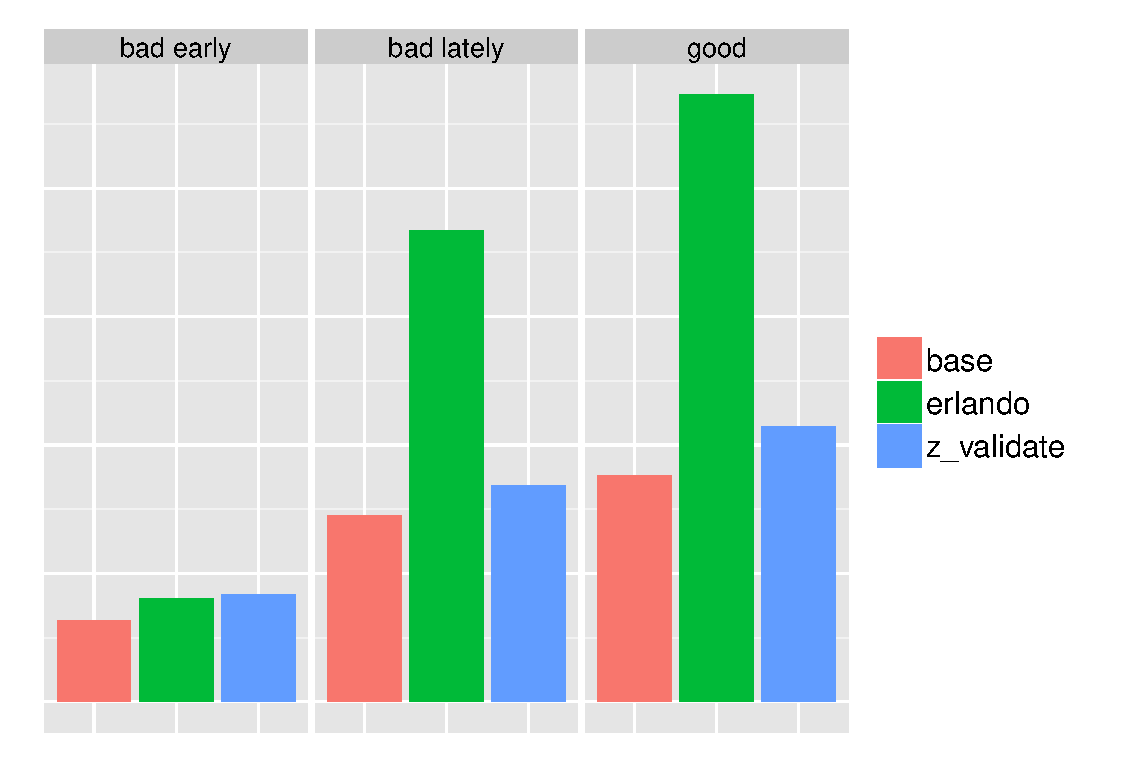
\includegraphics[scale=0.55]{plot.pdf}
  \end{center}
\end{frame}

\begin{frame}\label{lastframe}
  \begin{center}
    \Large
    Questions?\\\vspace{15pt}
  \end{center}
  Libraries:\\
  https://github.com/extend/sheriff\\
  https://github.com/rabbitmq/erlando\\
  https://github.com/si14/z\_validate\\
  Slides:\\
  https://github.com/si14/euc-2012-slides
\end{frame}
